\section{Visualisation des satellites}\label{sec:visualisation-des-satellites}
   Afin d'affiner notre compréhension du système GNSS, et nous aider à mieux le visualiser, déterminer l'origine des mesures en exploitant les données sur les satellites émetteurs nous a semblé indispensable.
   En effet, les constellations de satellites utiles au positionnement assurent continument un service de géolocalisation autour du monde.
   Ainsi, à tout moment, des satellites émettent des données pouvant être lues par un récepteur.

   Pour nous donner une petite idée de cette disponibilité des satellites, tracer depuis un fichier NMEA la position des satellites ayant servi au positionnement (trames GSV) nous semble être une manière intéressante de procéder.
   Il est alors nécessaire de pouvoir remonter des données brutes enregistrées par le récepteur à la position des satellites autour de la Terre.

   \subsection{Récupération des données}\label{subsec:recuperation-des-donnees}
      La première étape est donc d'extraire du fichier NMEA les information sur les satellites émetteurs.
      Pour cela, nous allons extraire les trames GSV et en extraire les informations, à savoir le nombre de satellites disponibles, et pour chacun sa position en azimut et élévation ainsi que la force du signal.
      La méthode \texttt{satellite\_pos} permet donc cette extraction des données en les organisant dans une matrice de transmission contenant toutes ces caractéristiques sur les satellites.

      \begin{figure}[h]
          \centering
          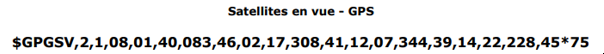
\includegraphics[width=.95\textwidth]{imgs/gsv}
          \caption{Exemple de trame GSV}
          \label{fig:gsv}
      \end{figure}

   \subsection{Tracé dans le référentiel de l'observateur}\label{subsec:trace-dans-le-referentiel-de-l'observateur}
      Une fois les données extraites, nous avons souhaité, dans un premier temps, positionner ces satellites dans une carte du ciel vue de la position du récepteur.

      Tout d'abord, les coordonnées horizontales sont converties en coordonnées sphériques locales centrées sur le récepteur GNSS\@.
      En effet, en orientant l'axe des abscisses vers l'Est, l'axe des ordonnées vers le Nord et les cotes vers les altitudes croissantes, on obtient une vue des satellites dans le ciel en faisant correspondre l'azimut avec l'angle $\pi/2 - \phi$ et l'élévation avec l'angle $\theta$.
      Le rayon $r$ sera déterminé arbitrairement.

       \begin{figure}[h]
             \centering
             \begin{subfigure}[h]{.45\textwidth}
                \centering
                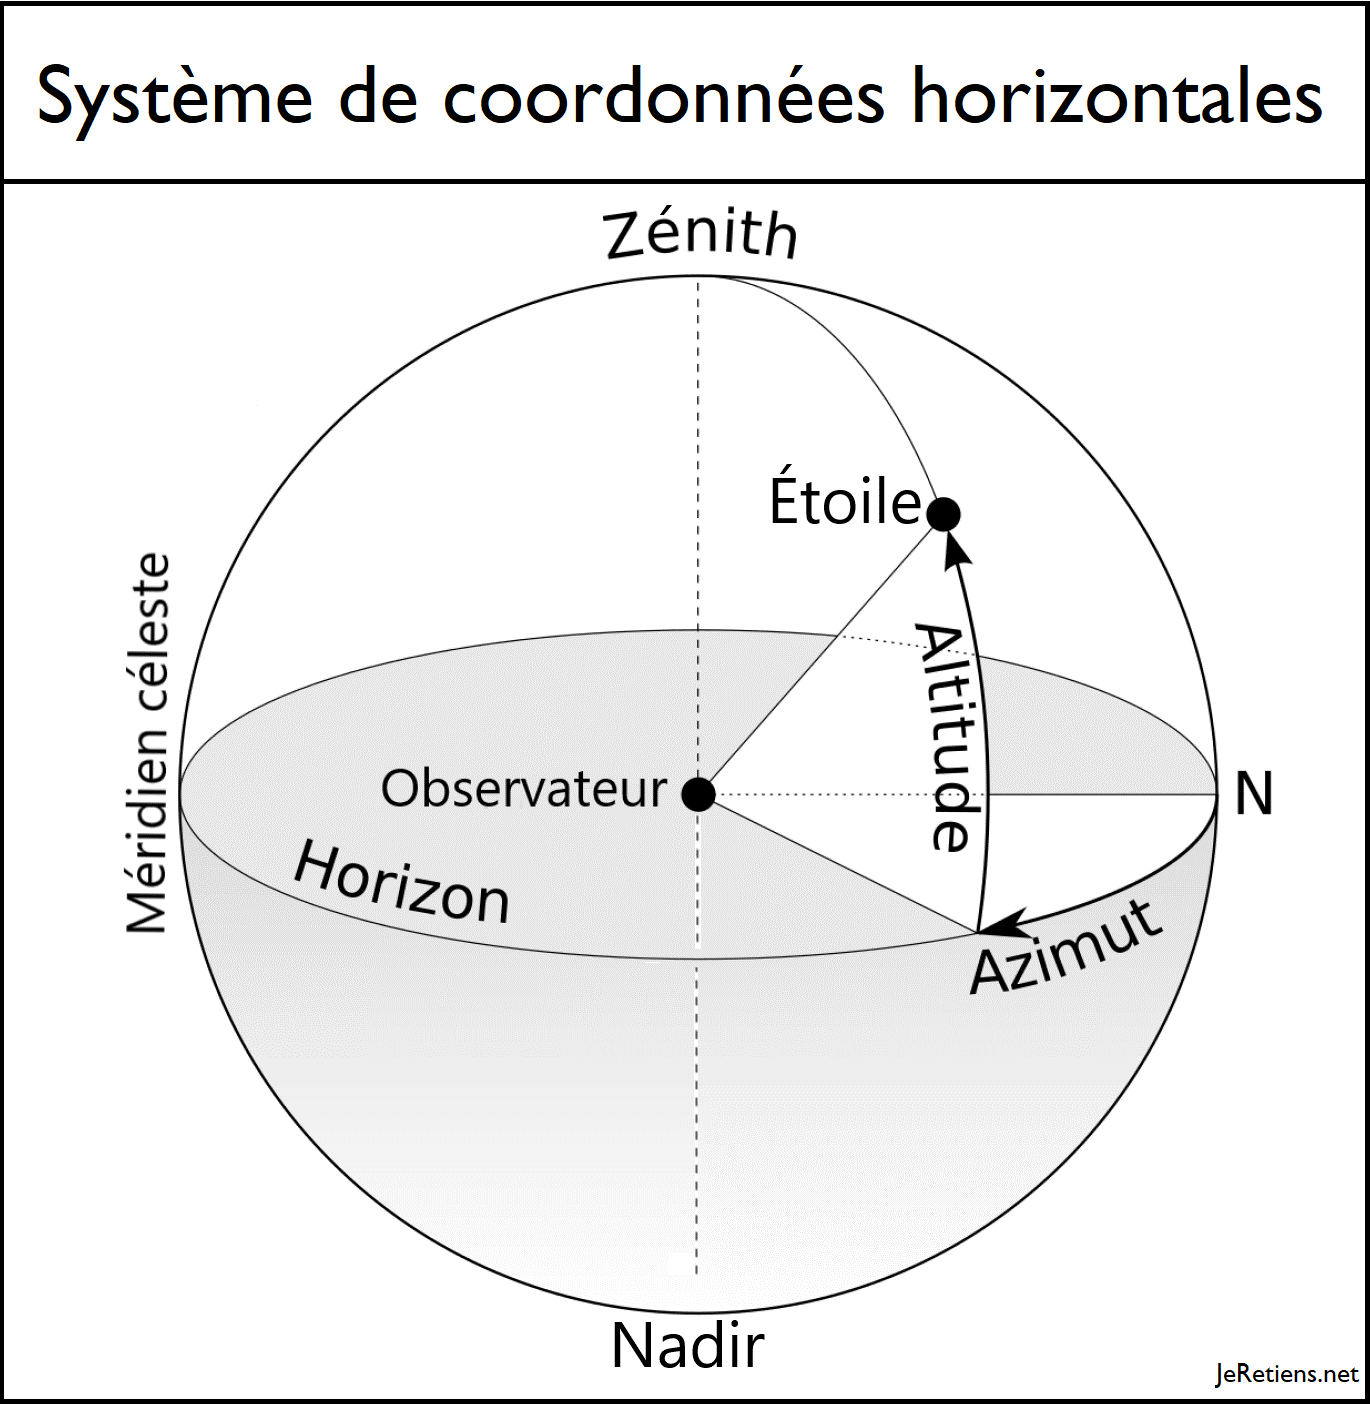
\includegraphics[width=\textwidth]{imgs/horizon}
             \end{subfigure}
             \hfill
             \begin{subfigure}[h]{.45\textwidth}
                \centering
                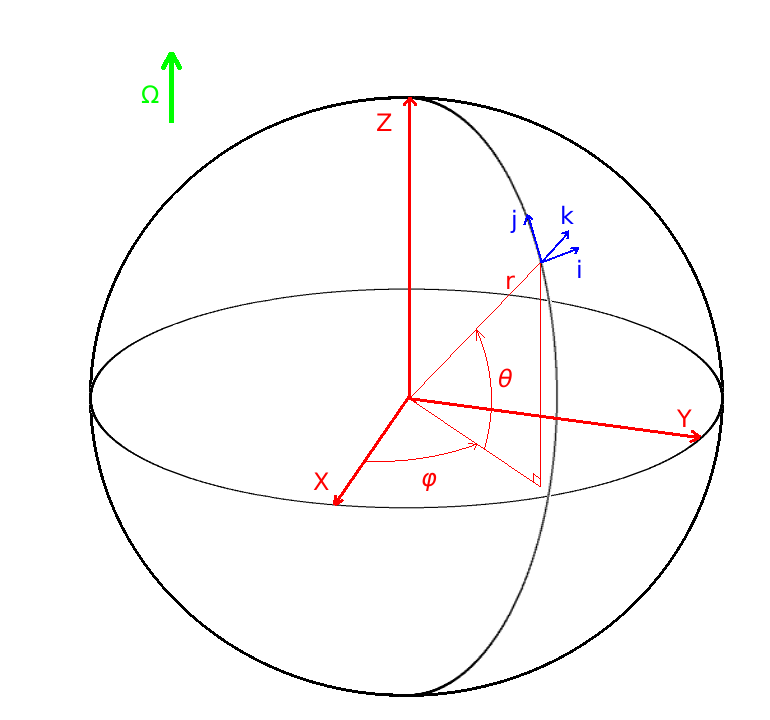
\includegraphics[width=\textwidth]{imgs/geo}
             \end{subfigure}
             \caption{Systèmes de coordonnées a) horizontales et b) géométriques}
             \label{fig:coords-terre}
         \end{figure}

      Puis, pour programmer le tracé dans Python, nous utilisons les coordonnées cartésiennes obtenues par :
      \[\begin{cases}
           x = r\sin\theta\cos\phi \\
           y = r\sin\theta\sin\phi \\
           z = r\cos\theta \\
      \end{cases}\]
      le tout réalisé par la méthode \texttt{plot\_satellite}.

      \begin{figure}[h]
          \centering
          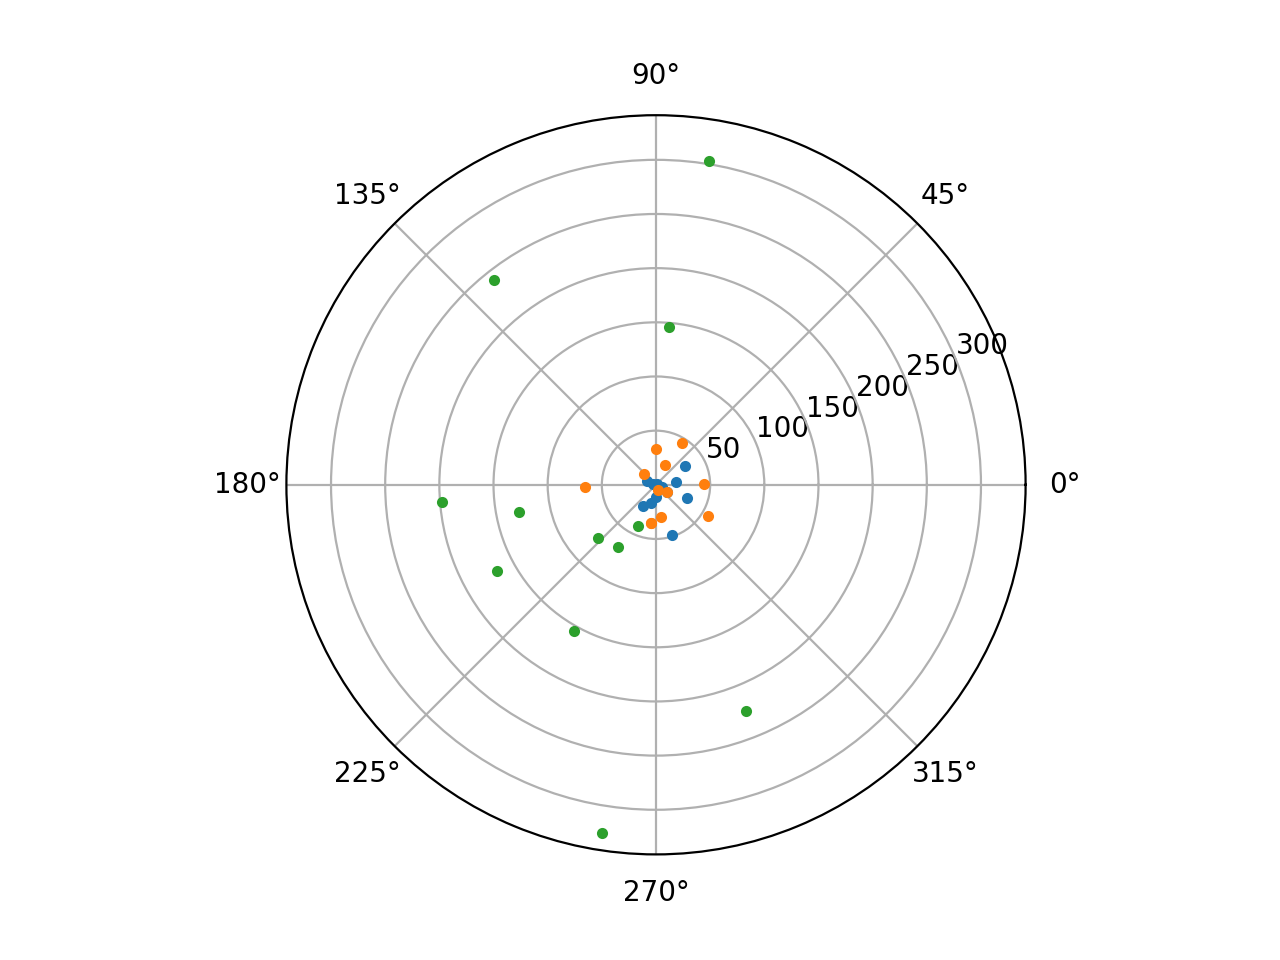
\includegraphics[width=.7\textwidth]{imgs/satpolar}
          \caption{Carte céleste des satellites}
          \label{fig:polarsat}
      \end{figure}

   \subsection{Tracé dans le référentiel géocentrique}\label{subsec:trace-dans-le-referentiel-geocentrique}
      Enfin, pour nous munir d'une représentation d'avantage complète et visuelle du positionnement des satellites en orbite, il nous a semblé judicieux de les placer dans le repère géocentrique.
      Il sera donc nécessaire de convertir les coordonnées horizontales obtenues précédemment.

      Nous devons donc effectuer la conversion du système de coordonnées ENU (\textit{East North Up}), qui est dans le plan local tangent à la Terre (correspondant au repère cartésien du système de coordonnées précédemment introduit) dans le système de coordonnées ECEF (\textit{Earth Centered Earth Fixed}) correspondant au repère cartésien géocentré.
      \begin{center}
         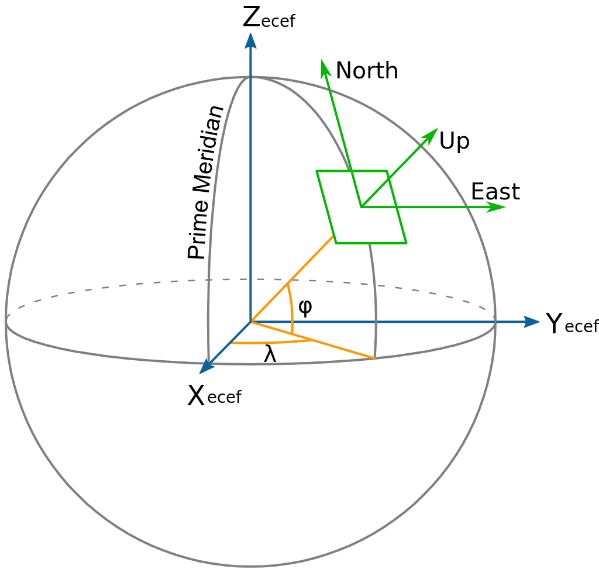
\includegraphics[width=.35\textwidth]{imgs/enutoecef}
      \end{center}

      La conversion est effectuée par le produit matriciel :
      \[
         \begin{pmatrix}
            X \\
            Y \\
            Z
         \end{pmatrix} =
         \begin{pmatrix}
            -\sin\lambda & -\sin\phi\cos\lambda & \cos\phi\cos\lambda \\
            \cos\lambda  & -\sin\phi\sin\lambda & \cos\phi\sin\lambda \\
            0            & \cos\phi             & \sin\phi
         \end{pmatrix}
         \begin{pmatrix}
            x \\
            y \\
            z
         \end{pmatrix}
      \]

      Grâce à la matrice de conversion, il est donc possible de déterminer les nouvelles coordonnées des satellites, puis de tracer en trois dimensions la position du récepteur sur la Terre, puis la position des satellites en orbite (d'altitude fixée arbitrairement pour la visualisation).

      \begin{figure}[h]
          \centering
          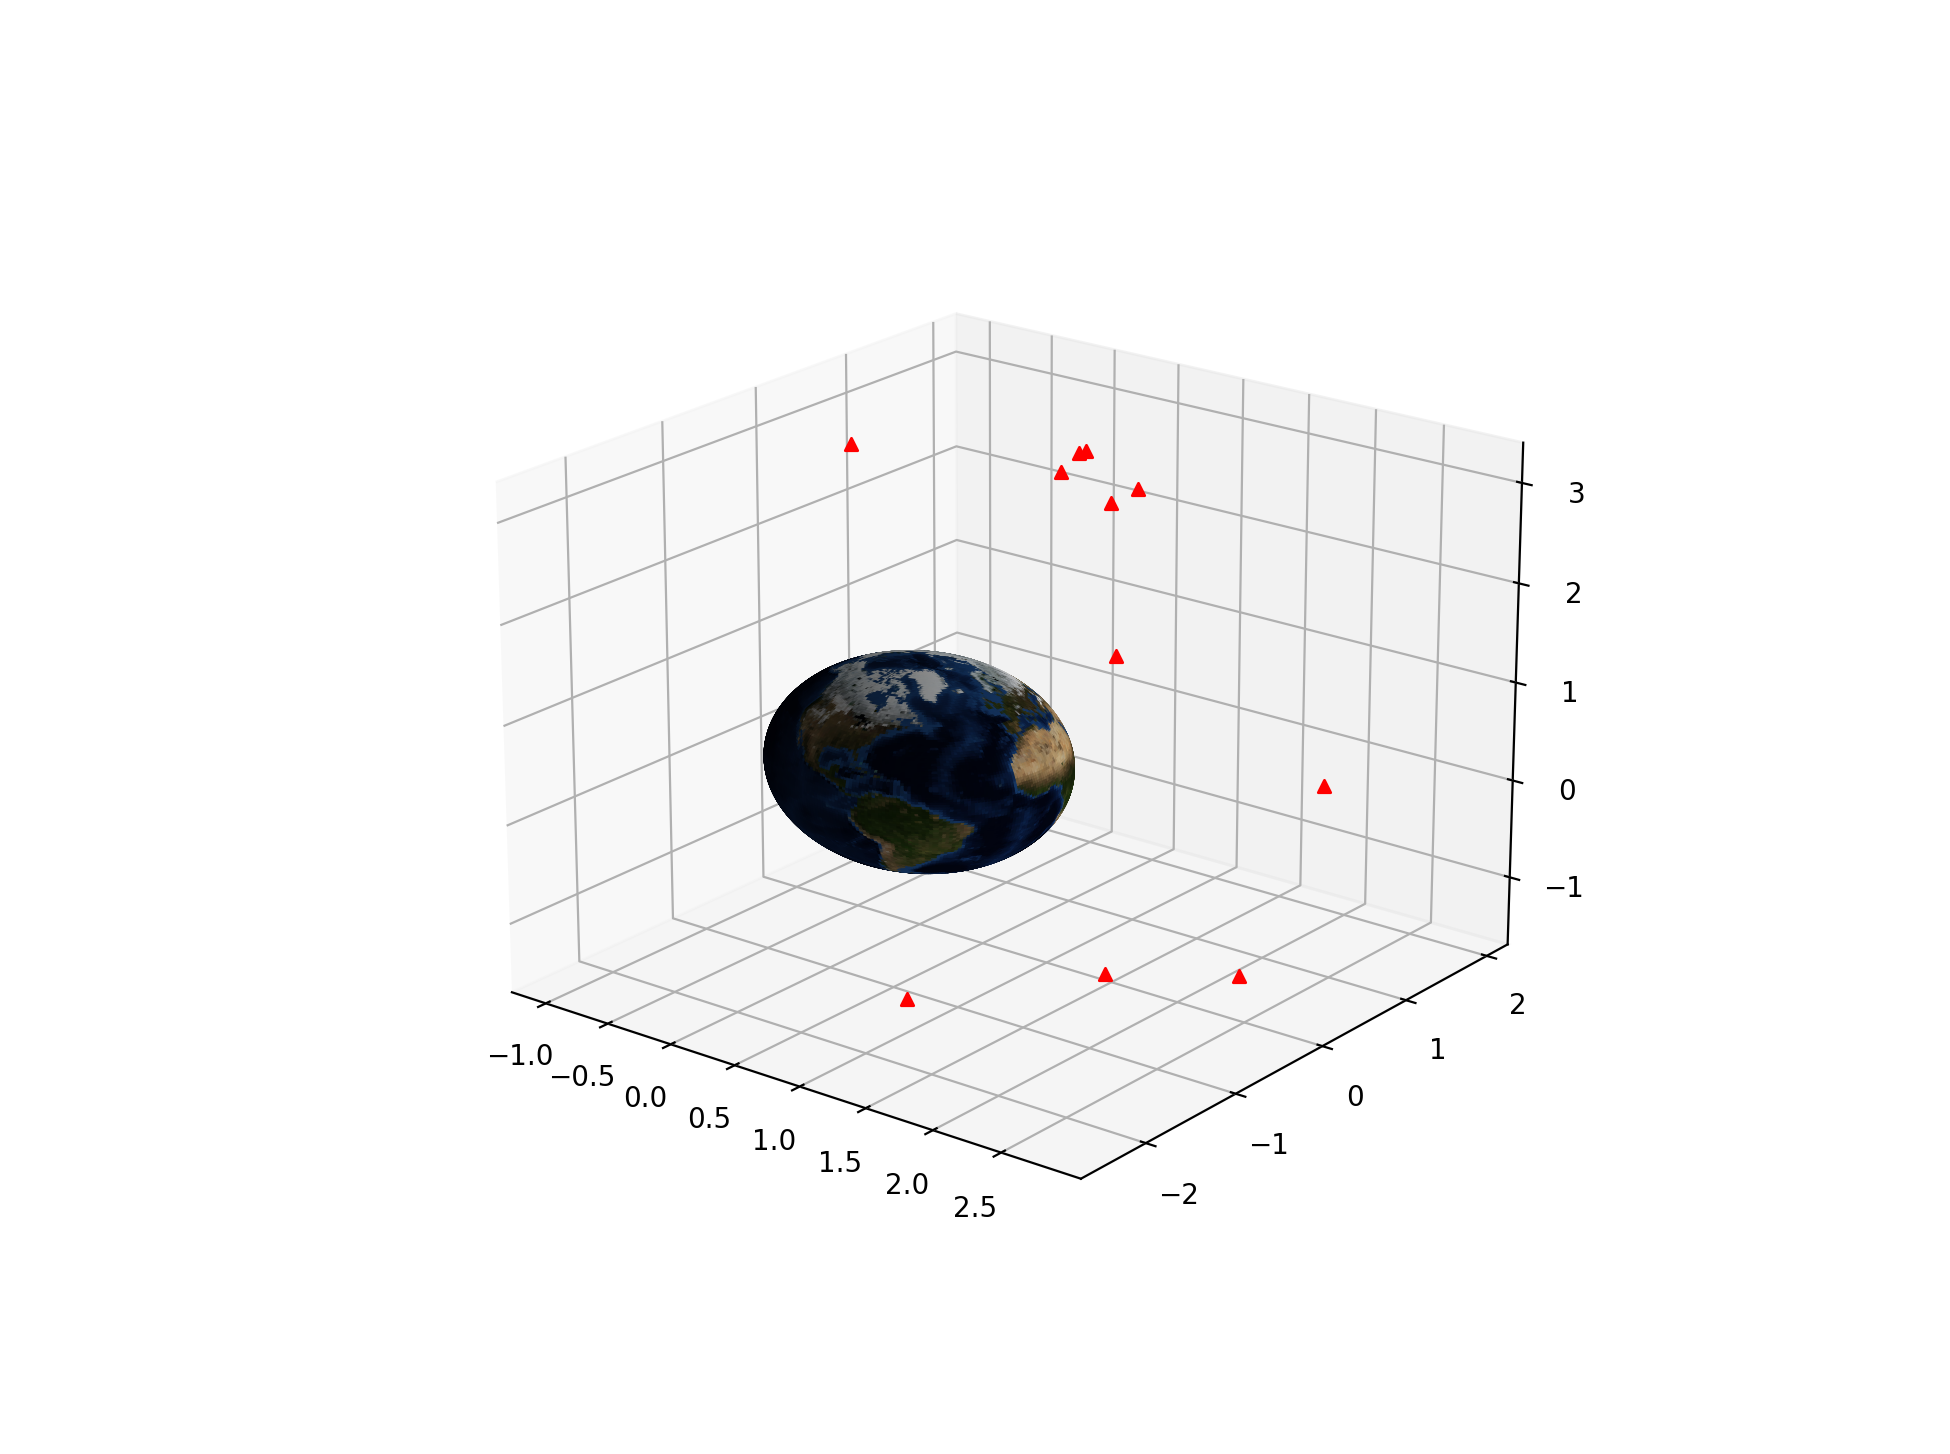
\includegraphics[width=.7\textwidth]{imgs/visuplanet}
          \caption{Résultat de la méthode \texttt{visu\_planet}}
          \label{fig:visuplanet}
      \end{figure}